\documentclass[11pts,english,letterpaper]{scrartcl}

\usepackage[utf8]{inputenc}
\usepackage[T1]{fontenc}
\usepackage{babel} 
\usepackage{amsmath}
\usepackage{amsfonts}
\usepackage{amssymb}
\usepackage{float}
\usepackage{geometry} 
\usepackage{rotating} 
\usepackage{graphicx}
\usepackage{xspace}
\usepackage{layout}
\usepackage{mathpazo}
\usepackage{microtype}
\usepackage{xcolor}
\usepackage{tabularx}
\usepackage{paralist}
\usepackage{setspace}
\usepackage{makeidx}
\usepackage{multirow}
\usepackage{booktabs}
\usepackage{lscape}

\makeindex

\usepackage[colorlinks,linktocpage]{hyperref}

\newcommand\ERR[3][]{$\left(#2 \pm #3\right) #1$}
\newcommand\ERRm[3][]{\left(#2 \pm #3\right) #1}
\newcommand\DIF[2][]{\frac{\text{d}#1}{\text{d}#2}}
\newcommand\grad[0]{{}^\circ}
\newcommand\srcfile[1]{\texttt{src/WCSim#1}}
\newcommand\volume[1]{\textsf{\textbf{#1}}}

\floatplacement{figure}{!htb}
\graphicspath{{./figures/}}


\author{Alexander Himmel, Johannes Hoppenau, Joseph Lozier}
\title{Simulating Water Cherenkov Detectors Using \texttt{WCSim}}

\graphicspath{ {figures/} }

\begin{document}
\maketitle
\tableofcontents

%===========================================

\section{Overview}

WCSim is a flexibile Geant4-based simulation of a water-Cherenkov detector with top and side photo-multiplier tubes.  Given basic parameters about the detector, it automatically lays out the PMTs so you can get started simulating events as soon as possible.  This document will describe the detector geometry and all its elements.  It describes how to set up a new custom detector and how to configure the simulation options.  Finally, it describes the ROOT output file and how to access the stored data with some simple examples.


\section{The WCSim Geometry}
The \texttt{WCSimDetectorConstruction::ConstructWC()} method returns a pointer to a logical volume that contains an upright cylindrical detector. The function is defined in \srcfile{ConstructWC.cc}. The inner detector consists only of blacksheet and PMTs, and the optional top veto outer detector contains only blacksheet, whitesheet, and PMTs.

The PMTs and the blacksheet are organized into cells along the cylinder walls plus a top and bottom cap. This structure makes it easy to add outer detector PMTs to the sides and bottom or a steel structure behind the blacksheet. The method is written generically, making it possible to simulate many different detectors. 

\subsection{Hierarchy of Volumes}
This section describes the the volumes that make up the detector. (Figure \ref{fig:hi})
\begin{figure}[b!]
  \begin{center}
  \includegraphics[width=0.40\textwidth]{expHall2} 
  \hspace{0.1\textwidth}
  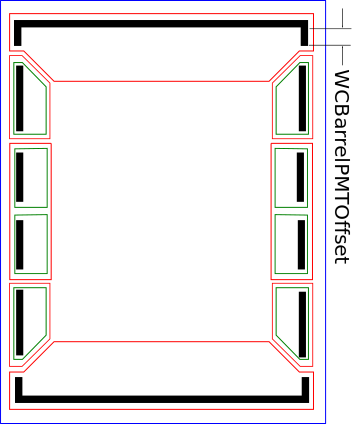
\includegraphics[width=0.40\textwidth]{annulus}
  \end{center}
  \caption{On the left is a 3D schematic of the cylindrical detector and on the right is a 2D cross-section that better shows the volume hierarchy contained in \volume{WCBarrel}.  The outermost level is \volume{ExpHall} (dotted black line) which is an air-filled rectangle.  It contains \volume{WC} (narrow black line), the volume returned by \texttt{WCSimDetectorConstruction::ConstructWC()}.  Inside it is the water-filled cylinder \volume{WCBarrel} (blue) whose sub-volumes are labeled on the right and described in the text below.}
%It contains \vol{WCBarrelAnnulus}, the main part of the walls of the detector, and the the two \voume{WCCapAssembly}'s (yellow).  \vol{WCBarrelAnnulus} contains \volume{WCBarrelRing}'s which are themselves divided up into \vol{WCBarrelCell}'s (green), which in turn contain \volume{WCPMTs}.  The \volume{WCCapAssembly}'s contain the \volume{WCBarrelAnnulus}, \volume{WCBarrelBorderRing} and  \volume{WCCap} (red) are the volumes the are divided into the cells (green) that hold the PMTs (not pictured) and the blacksheet (thick black line).  \volume{WCCapAssembly} (yellow) contains \volume{WCBarrelBorderCell} and  \volume{WCPMTCap}.  Note that colors refer to both persective and section views.}
\label{fig:hi}
\end{figure}


\begin{description}
  \item[ExpHall] is the world volume. It is not constructed in  \srcfile{ConstructWC.cc} but in \srcfile{DetectorConstruction.cc}.
  \begin{description}
    \item[WC] is a tubs filled with air. At the moment it  only contains one daughter volume:
    \begin{description}
      \item[WCBarrel] is a tubs filed with water. It contains all of the current detector structure (PMTs and blacksheet), divided into the annulus and the caps:
      \begin{description}
        \item[WCBarrelAnnulus] is the main part of the detector wall. It is divided into rings:
        \begin{description}
          \item[WCBarrelRing] each one cell high, which are then divided into cells:
          \begin{description}
            \item[WCBarrelCell] These cells contain one or more PMTs (\volume{WCPMT}'s) and the blacksheet (\volume{WCBarrelCellBlackSheet}).  Each cell is flat and represents one modular detector section.
          \end{description}
        \end{description}
        \item[WCTopCapAssembly and WCBottomCapAssembly] are two mirrored volumes that close the ends of the barrel.  They are constructed by calling \srcfile{WCSimDetectorConstruction::ConstructCaps(G4int zflip)}, where the argument, zflip, equals 1 to generate the \volume{BottomCapAssembly} and -1 to generate the \volume{TopCapAssembly}.  This method allows symmetric changes to the caps by editing ConstructCaps and avoids using Geant's built-in ReflectionFactory, which is incompatible with the OpticalSurface used to model certain PMT properties.
        \begin{description}
          \item[WCCap] This volume contains all of the cap PMTs (\volume{WCPMT}) and the blacksheet behind them (\volume{WCCapBlackSheet}) which extends around the cylinder edges to connect to:
          \item[WCBarrelBorderRing] This volume connects the annulus to the cap.  It is essentialy the uppermost (or lowermost) ring of PMTs, but has a modified  bounding-box geometry and is contained in the CapAssembly because it must mate at the corner with the caps.  (N.B.  See \ref{sec:warnings}, for information on corner geometry.)  The border ring is divided into cells:
          \begin{description}
            \item[WCBarrelBorderCell] that contain the same number of PMTs (\volume{WCPMT}) and the same blacksheet (\volume{WCBarrelCellBS}) as the normal annulus cells.
          \end{description}
        \end{description}
        \item[WCExtraTower] is a tower that is narrower than the normal cells that is added if the number of PMTs circumferentially is not divisible by the number of PMTs horizontally in each cell.  It is divided into cells:
        \begin{description}
            \item[WCExtraTowerCell] that contains the remaining PMTs (\volume{WCPMT}) and blacksheet  (\volume{WCTowerBlackSheet}) (figure \ref{fig:extra}).  The cap assemblies conatin a corresponding this corresponding extra cell called \volume{WCExtraBorderCell}.
        \end{description}
      \end{description}
    \end{description}
  \end{description}
\end{description}      



\volume{WCPMT} is a single cylindrical volume containing a single PMT model that is placed many times in the detector.  The volume is described in \srcfile{WCSimConstructPMT.cc}.  The surrounding volume is cylindrical with a coordinate origin where its axis intersects the blacksheet (not a standard tubs) (red box, \ref{fig:pmt}).  The PMT is made up of two sub-volumes, both spherical caps: the hollow glass outer face of the PMT (\volume{GlassFaceWCPMT}) and the inner vacuum (\volume{InteriorWCPMT}).  The optical inner coating of the PMT glass is modeled as an OpticalSurface (not a volume) (\volume{GlassCathodeSurface}) between the glass and vacuum.  (See also \ref{fig:pmt}.)  Any components added to this single volume (e.g., an acrylic pressure vessel) are replicated and placed along with every PMT.


\begin{figure}[p]
   \begin{center}
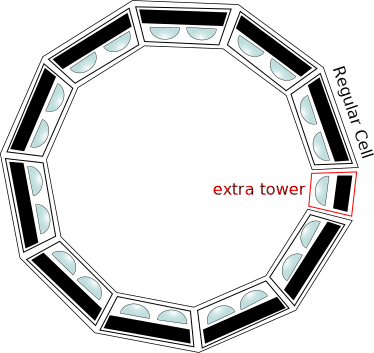
\includegraphics[width=0.60\textwidth]{extraTower} 
  \end{center}
\caption{If the number of PMTs in one cell (in this example, 2) does not divide the total number of PMTs in one ring (in this example, 2), there is an extra tower that contains the remaining PMTs}\label{fig:extra}
\end{figure}

\begin{figure}[p]
  \begin{center}
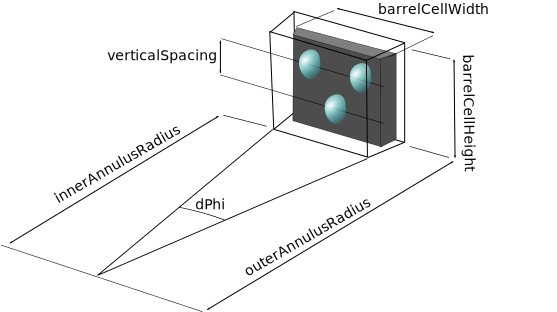
\includegraphics[width=0.60\textwidth]{Cell}
  \end{center}
\caption{Each cell holds blacksheet and multiple PMTs. All labeled lengths are calculated automatically. In the current version, the PMTs are distributed equally in horizontal and vertical direction.}
\end{figure}


%============================================

\section{Setup your own detector}

The dimensions of the detector to be setup must be described in member variables of  \texttt{WCSimDetectorConstruction} before calling  \texttt{WCSimDetectorConstruction::ConstructWC()}. This section describes which geometric parameters must be set. The easiest and least error-prone way to to set the variables is to add a method to the \texttt{WCSimDetectorConfigs.cc} file that is a copy of an existing detector configuration with the necessary changes.
You can either call this function in the constructor of \texttt{WCSimDetectorConstruction} or add it to the detector messenger (\srcfile{DetectorMessenger.cc}) if you want call it in a macro file or you want to change the detector setup dynamically. If you want to do this, you first have to use the command that calls your function (\texttt{/WCSim/WCgeom <geometry name>}) to set the parameters, and afterwards the detector construction command (\texttt{/WCSim/Construct}) to (re)construct the geometry.

\subsection{Parameters}\label{sec:param}
To set up a new detector geometry the following parameters must be set:

\begin{figure}
  \begin{center}
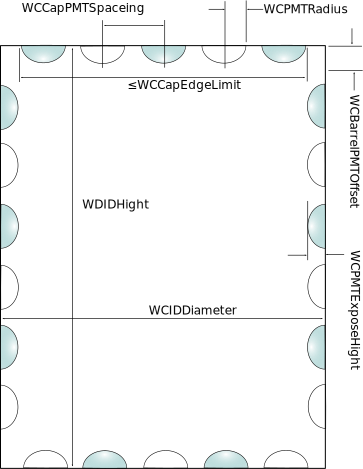
\includegraphics[width=0.60\textwidth]{variables}
  \end{center}
\caption{These are among the variables you have to set to create a new detector geometry.}\label{fig:geom}
\end{figure}


\begin{description}
\item[PMTName] selects a PMT quantum efficiency model.  Supported names are "10inch", "10inchHQE" and "20inch".

\item[WCPMTRadius, WCPMTExposeHeight] (see figure \ref{fig:pmt}) are the radius at blacksheet and height above blacksheet, respectively, of the PMTs. Note that the digitizer recognizes PMT models by radius to determine a timing constant, so diameter configuration is limited to know sizes. Supported diameters are 8, 10, 12 and 20 inches (1016, 1270, 1524 and 2540 mm radii, respectively).

\begin{figure}
  \begin{center}
    
\includegraphics{PMT}
  \end{center}
\caption{The PMTs are segments of spheres.  All parts are contained in the bounding cylinder, \volume{WCPMT} (red).  The PMT glass (\volume{GlassFaceWCPMT}, blue) and the sensitive volume, the inner vacuum (\volume{InteriorWCPMT}, green) are contained within. Also present is the optical coating between the glass and vacuum (\volume{GlassCathodeSurface}, yellow).  To define the geometry of the PMTs you need to set the \texttt{WCPMTGlassThickness}, the \texttt{WCPMTRadius}, and the \texttt{WCPMTExposeHight}}\label{fig:pmt}
\end{figure}

\item[WCIDDiameter, WCIDHeight] These two variables are used to setup the size of the detector. The height is the distance between the inner surfaces of the top and bottom blacksheets and the diameter is two times the shortest distance between the inner surface of the wall blacksheet and the center of the detector (see figure \ref{fig:geom}).  This shortest radius occurs at the center of normal (not extra) cells, and is perpendicular to the blacksheet.

\item[WCBarrelPMTOffset] The cap volumes contain vertical space in stripes along the edges of the detector to make room for the cap PMTs (N.B.  See \ref{sec:warnings}, for information on corner geometry). This variable defines the width of these stripes.  Specifically, the offset is the vertical distance from the inner surface of the cap blacksheet to the upper edge of the top cell.  This edge is half the vertical PMT spacing vertically above the center of each PMT in the uppermost (or lowermost) ring.

\item[WCPMTperCellHorizontal, WCPMTperCellVertical] are two integers that define the arrangement of PMTs within each cell, the product of which gives the number of PMTs in each cell.

\item[WCBarrelNumPMTHorizontal] defines the number of PMTs circumferentially around the detector. If WCPMTperCellHorizontal does not divide this number, there will be an extra cell in each ring, which contains the remaining PMTs.

\item[WCBarrelNRings] defines how many rings of cells there will be vertically.  The total number of PMTs in a vertical column will be the product of this number and WCPMTperCellVertical.

\item[WCCapPMTSpacing] defines the center-to-center spacing of the PMTs on the top and the bottom caps of the detector.

\item[WCCapEdgeLimit] is the maximum distance between the center of the cap and the outer edge of a cap PMT (the edge is WCPMTRadius away from the center of the PMT, whose coordiantes on the cap are half-integer multipules of WCCapPMTSpacing). This length has to be smaller than half the \texttt{WCIDDiameter}. Otherwise there may be PMTs that intersect the edge of the caps.  The WCSimConstructWC places PMTs on the caps in a grid subject only to this constraint.  Note that the four centermost cap PMTs are equidistant from the cylinder axis.

\item[WCPMTGlassThickness] the thickness of the glass face.

\item[WCBlackSheetThickness] the thickness of the blacksheet.

\item[WCAddGd] a boolean that, when true, dopes the water volume with .01\% Gadolinium by mass.
\end {description}

All other values needed to set up the geometry are derived from these variables.

\subsection{Example}

\begin{lstlisting}
void WCSimDetectorConstruction::SetSuperKGeometry()
{
  WCPMTName             ="20inch";
  WCPMTRadius           =.254*m;  
  WCPMTExposeHeight     =.18*m; 
  WCIDDiameter          = 33.6815*m;//16.900*2*
                                    //cos(2*pi*rad/75)*m;
  WCIDHeight            = 36.200*m;
  WCBarrelPMTOffset     = 0.0715*m; //offset from vertical
  WCBarrelNumPMTHorizontal  = 150; 
  WCBarrelNRings        = 17.;
  WCPMTperCellHorizontal= 4;
  WCPMTperCellVertical  = 3; 
  WCCapPMTSpacing       = 0.707*m; // distance between centers
                                   // of top and bottom pmts
  WCCapEdgeLimit        = 16.9*m;
  WCPMTGlassThickness   = .4*cm;
  WCBlackSheetThickness = 2.0*cm;
  WCAddGd               = false;
}
\end{lstlisting}

This is the Super-K setup. This method is located at the beginning of \srcfile{ConstructWC.cc}. It is called in the constructor of \texttt{WCSimDetectorConstruction}.
In SK the PMTs are arranged in $4 \times 3$ cells (\texttt{WCPMTperCellHorizontal} and \texttt{WCPMTperCellVertical}). 
All in all there are 51 rings of PMTs (3 lines in each cell times 17 lines of cells (\texttt{WCBarrelNRings})). Each line contains 150 PMTs (\texttt{WCBarrelNumPMTHorizontal}). As 150 divided by 4 is 37.5, there are 37 regular $4 \times 3$ cells and one $2 \times 3$ cell in one ring.  Note that Super-K's plans specify a 16.9 meter radius to the corner between cells, some triginometry was required to translate this to a perpendicular distance, almost 6 cm less.

The vertical spacing of the PMTs is
\[
\frac{\texttt{WCIDHeight} - 2\cdot\texttt{WCBarrelPMTOffset}}
{\texttt{WCBarrelNRings} \cdot \texttt{WCPMTperCellVertical}}
= 0.707 \mathrm{m}.
\]
between the bottom (and top) blacksheet and the cells on the wall, there is a gap of 7.15 cm (\texttt{WCBarrelPMTOffset}).

The caps are completely filled with PMTs, because \texttt{WCCapEdgeLimit} is equal to the detector diameter. 



\subsection{Warnings}
If the PMTs have a large \texttt{WCPMTExposeHeight} and there is not enough space between the PMTs and the borders of the cells, the PMTs could intersect the edge of the border cells, because the border of these cells are slanted (see figure \ref{fig:warning}).
\label{sec:warnings} 

This can also happen at the caps if \texttt{WCCapEdgeLimit} is close to the inner radius of the detector and \texttt{WCBarrelPMTOffset} is small.

\begin{figure}[t]
  \begin{center}
\includegraphics{warning}
  \end{center}
\caption{The topmost and bottommost PMTs could  intersect the border of the cells.} \label{fig:warning}
\end{figure}

During the setup an incomplete checking for obvious overlaps occurs. You should see a lot of the flowing lines:\\
\texttt{Checking overlaps for volume WCBarrelPMT ... OK!}\\
If you see warnings instead, it is likely that there are too large or too many PMTs.  An absence of warnings does not mean that there are no overlaps.

There is no check if the placement of the PMTs on caps is correct. It would take to much time to do this check every time, because there are too many PMTs in side a single volume.

Some rules of thumb to avoid overlaps are: \texttt{WCBarrelPMTOffset > WCPMTExposeHeight} or \texttt{WCIDDiameter / 2 - WCCapEdgeLimit > WCPMTExposeHeight} ensures cap PMTs are fully within the cap volume, and \texttt{vertical spacing of the PMTs / 2 > WCPMTExposeHeight + WCPMTRadius} ensures the top and bottom ring PMTs are within \volume{WCBarrelBorderRing}.  These rules are general, and PMTs may be placed closer with careful attention to geometry.  Collisions are not an issue in Super-K, and newer detectors with smaller, more-efficient (and thus sparser) PMTs should have little issue provided reasonable specifications of \texttt{WCCapEdgeLimit} and \texttt{WCBarrelPMTOffset}.
 
 

\subsection{Input Files}

Some tuning paramters are found in \texttt{jobOptions.mac} and \texttt{tuning\_parameters.mac}, which are in seperate files because they must be loaded at specific times during initialization.  The bulk of options, however, may be found in \texttt{vis.mac}, the default inupt file.  WCSim is a GEANT4 program  and accepts GEANT4 commands as an input file or at runtime.  GEANT documentation describes the commands not detailed here.
\begin{description}
\item[/WCSim/WCgeom] selects a set of geometry parameters (see \ref{sec:param}.)  It does not create a new geometry.  Availible arguments include \texttt{SuperK} and \texttt{DUSEL\_200kton\_12inch\_HQE\_10perCent}.  New geometries are easily added and a full list of those already available may be found in \srcfile{DetectorMessenger.cc}
\item[/WCSim/Construct] constructs the detector geometry in memory based on the previously selected parameters.  Takes no arguments.
\item[/WCSim/WCPMTsize] options are \texttt{10inch} and \texttt{20inch}.  Refers to models of PMT quantum efficieny.
\item[/WCSim/PMTQEMethod] Selects the quantum efficiency method. Possible arguments are: \texttt{Stacking\_Only}, in which the QE is applied to reduce the total number of photons when the photons are generated; \texttt{Stacking\_And\_SensitiveDetector}, which the (constant) QE at the most efficient wavelength is applied at photon creation, then the remaining (wavelength-dependent) loss is applied at the detector; and \texttt{SensitiveDetector\_Only}, in which QE is applied at the detector only.
\item[/WCSim/PMTCollEff] Selects wavelength-dependent (\texttt{on}) or -independent (\texttt{off}) quantum efficiency model.
\item[/WCSim/SavePi0] Selects whether or not Pi0-specific information is saved, options are \texttt{true} and \texttt{false}.

\end{description}



\section{Output Root File}

\begin{figure}[t!]
  \begin{center}
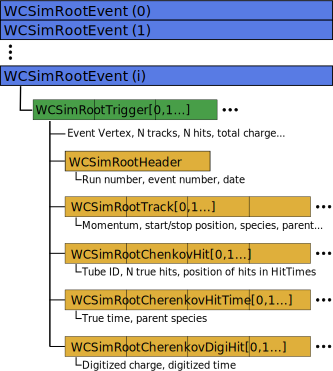
\includegraphics{rootfile}
  \end{center}
\caption{The class hierarchy of the WCSimRootEvent written to the output file.} \label{fig:rootfile}
\end{figure}

WCSim writes the results of the simulation in a root file. You can set the name and path of this file in the \texttt{vis.mac} file using the \texttt{/WCSimIO/RootFile} command.  To read from the root file, the command \texttt{gSystem.Load("<\emph{WCSim Directory}>/libWCSimRoot.so")} should be run in root to load shared classes.  This shared object library is created by running "gmake shared" on the command line.

A typical analysis will loop through events (one per simulated initial vertex), and in each event loop through the observed triggers (sually one for the initial particles and sometimes additional triggers for delayed decay products).  In each tigger, you access a list of digitized hits, each containing the charge, time, and ID of the hit PMT.  To get the location of the hit, you use the geometry object to access the PMT object that corresponds to that Tube ID.  This structure avoids having to store a list containing every PMT in every sub-event.

The files \texttt{sample-root-scripts/read\_PMT.C} and \texttt{sample-root-scripts/testgeo.C} provide general examples for how to read \texttt{wcsimT} and \texttt{wcsimGeoT}, and are probably the best starting point for custom analysis.  There is also some annotated example code in the next subsection.


\subsection{The Class Hierarchy}

The root file itself contains 2 \texttt{TTree}s, each with only 1 branch containing a custom object: \texttt{wcsimT} with branch \texttt{wcsimrootevent} and \texttt{wcsimGeoT} with branch \texttt{wcsimrootgeom}.  The first has an entry corresponding to each GEANT event and contains the truth and hit data, while the second has only 1 entry which contains the geometry information for the simulated detector.  Below is a description of the class hierarchy for these two objects.

\begin{description}
  \item[WCSimRootEvent] is a container for the observed triggers. It always contains at least 1 trigger (number 0) which contains the information about the initial particle tracks given to GEANT.  If there are delatyed decay particles, these ``sub-events'' are added as additional triggers numbered from 1 onwards.  
  \begin{itemize}
  \item \texttt{GetTrigger(int i)} - Return trigger number \texttt{i}, a \texttt{WCSimRootTrigger*}
  \item \texttt{GetNumberOfEvents()} - Total observed triggers
  \item \texttt{GetNumberOfSubEvents()} - Number of sub-event triggers (\texttt{GetNumberOfEvents()-1})
  \item \texttt{HasSubEvents()} - Return true if there is more than 1 trigger
  \end{itemize}

  \begin{description}
    \item[WCSimRootTrigger] Container for all the information assosciated with a single trigger
    \begin{itemize}
    \item \texttt{GetHeader()} - return the header with run and event numbers, etc.
    \item \texttt{GetPi0Info()} - return Pi0 information if it was set to be stored in the mac file
    \item \texttt{GetMode()} - interaction mode code number
    \item \texttt{GetVtx(int i)} - event vertex, 0=x, 1=y, 2=z
    \item \texttt{GetNpar()} - number of true particles

    \item \texttt{GetNtrack()} - number of true particle tracks
    \item \texttt{GetTracks()} - TClonesArray of true particle tracks

    \item \texttt{GetNumTubesHit()} - number of tubes with a true hit
    \item \texttt{GetNcherenkovhits()} - number of true chereknov hits (quantum efficiency is already applied)
    \item \texttt{GetCherenkovHits()} - true PMT hits in each PMT (quantum efficiency is already applied)
    \item \texttt{GetCherenkovHitTimes()} - the true times of all the cherenkov hits (quantum efficiency is already applied)

    \item \texttt{GetNcherenkovdigihits()} - number of digitized hits
    \item \texttt{GetSumQ()} - sum of digitized charge
    \item \texttt{GetCherenkovDigiHits()} - digitized hits e.g. charge read out by the simulated electronics 
    \end{itemize}

    \begin{description}
      \item[WCSimRootHeader] is a simple container for the run number, event number, and date of the event.
      \item[WCSimRootTrack] is a true track of a particles generated in the simulation. It contains all the information about the track, like particle species, mass, momentum, the start and top volumes, and the parent species.  In each trigger the number of tracks is given by \texttt{GetNTrack()}.  %Each track contains the methods: \volume{GetIpnu()}, \volume{GetFlag()}, \volume{GetM()}, \volume{GetP()}, \volume{GetE()}, \volume{GetStartvol()}, \volume{GetStopvol()}, \volume{GetDir(i)}, \volume{GetPdir(i)}, \volume{GetStop(i)}, \volume{GetStart(i)}, \volume{GetParenttype(i)}, \volume{GetTime()}, \volume{GetId()}.
      \item[WCSimRootCherenkovHit] These hits are records of photons hitting the PMTs before the digitization step (and associated threshold, etc.). In each trigger the number of true cherenkov hits is given by \texttt{GetNcherenkovhits()}.
          \begin{itemize}
          \item \texttt{GetTotalPe(0)} - the position in the array of HitTimes
          \item \texttt{GetTotalPe(1)} - the number of true photons that hit this PMT, which is also the number of entries in that list that belong to this PMT
          \item \texttt{GetTubeID()} - tube id number
          \end{itemize}
      \item[WCSimRootCherenkovHitTime] This list stores the true time and parent ids of each cherenkov photon.  So, by looking up the photons assosciated with a particular PMT as above, the particles which contributed light to a particular phototube can be determined.
          \begin{itemize}
          \item \texttt{GetTruetime()} - true time of the hit
          \item \texttt{GetParentID()} - ID number of parent, allowing each photon to be traced to a specific true particle
          \end{itemize}
      \item[WCSimRootCherenkovDigiHit] These hits are the final output of the simulation. In each trigger the number of digitized hits is given by \texttt{GetNcherenkovdigihits()}.  The charge and time variables are those returned by the simulated electronics.
          \begin{itemize}
          \item \texttt{GetQ()} - the total charge measured by the PMT
          \item \texttt{GetT()} - the measured time of the hit
          \item \texttt{GetTubeId()} - ID number of the PMT
          \end{itemize}
    \end{description}
  \end{description}
\end{description}


\begin{description}
  \item[WCSimRootGeom]  has methods \texttt{GetWCCylRadius()}, \texttt{GetWCCylLength()}, \texttt{GetWCPMTRadius()} and \texttt{GetWCNumPMT()}, which return, respectively, the radius and length of the detector cylinder, the PMT radius, and the total number of PMTs.  The class can also return PMT objects by tube number via \texttt{GetPMT(i)}.
    \begin{description}
    \item[WCSimRootPMT] contains information for each PMT in the detector.
    	\begin{itemize}
                \item \texttt{GetTubeNo()} - the tube ID.
		\item \texttt{GetCylLoc()} - 0 for a PMT on the top cap, 2 for a PMT on the bottom  cap, and 1 for a PMT for a wall PMT.
		\item \texttt{GetPosition(j)} - where j is 0, 1, or 2.  Returns the x, y, and z coordinates of the center of the sphere that forms the PMT.
		\item \texttt{GetOrientation(j)} - where j is 0, 1, or 2.  Returns the x, y, and z components of the vector describing the direction the PMT faces.
         \end{itemize}
    \end{description}
\end{description}


\subsection{How to Use the Files}

%\newenvironment{code}{\begin{verbatim}}{\end{verbatim}}



There are example scripts showing how to use the root files in sample-root-scripts, but here are the basics of how to get the information out of the root file.

First, you need to load the root library into memory and assign the two WCSim branches:
\begin{lstlisting}
gROOT->Load("libWCSimRoot.so");

TTree  *wcsimT = f->Get("wcsimT");
WCSimRootEvent *wcsimrootevent = new WCSimRootEvent();
wcsimT->SetBranchAddress("wcsimrootevent",&wcsimrootevent);

TTree  *wcsimGeoT = f->Get("wcsimGeoT");
WCSimRootGeom* wcsimrootgeom = new WCSimRootGeom();
wcsimGeoT->SetBranchAddress("wcsimrootgeom",&wcsimrootgeom);  
wcsimrootgeom->GetEntry(0);
\end{lstlisting}

Since the geometry tree has only one entry, you may as well load it right away.  You loop through the events as with any root tree.   However, to get at any real information from the events, you will need to load the triggers.  The first trigger contains the main event information so here we will only load the first trigger.  Then from the trigger we can load and loop through all the digitized hits.

\begin{lstlisting}
wcsimT->GetEntry(ev);
WCSimRootTrigger *wcsimroottrigger =  wcsimrootevent->GetTrigger(0);

int ncherenkovdigihits =  wcsimrootevent->GetNcherenkovdigihits(); 
// Loop through elements in the TClonesArray
for (int i=0; i<ncherenkovdigihits; i++) {
    WCSimRootCherenkovDigiHit *hit = (WCSimRootCherenkovDigiHit*)
        (wcsimrootevent->GetCherenkovDigiHits()->At(i));

    double charge = hit->GetQ();
}
\end{lstlisting}

If you want to know the position of the hit we extracted above, we use the geometry tree to look up that information based on the TubeID.

\begin{lstlisting}
    int tubeId = hit->GetTubeId();
    WCSimRootPMT pmt = wcsimrootgeom->GetPMT(tubeId);
    double pmtX = pmt.GetPosition(0);
    double pmtY = pmt.GetPosition(1);
    double pmtZ = pmt.GetPosition(2);
\end{lstlisting}

%\subsection{root2zbs and superscan}
%To view the results of the simulation with superscan, you have to convert it into a zbs file first. To do this use \texttt{root2zbs <input file> <output file>}.

%To open this file with superscan you need the \texttt{geofile.txt} WCSim produces and a special version of superscan that can read in this file. In this file the positions and orientations of all PMTs and the size of the detector is stored. To let superscan know that there is a geofile, you have to set the \texttt{G4GEOFILE} environment variable to the path of this file.


\end{document}



